\documentclass[25pt,
margin=0mm, innermargin=15mm, blockverticalspace=5mm, colspace=15mm, subcolspace=1mm]{tikzposter}
\geometry{paperheight=42in,paperwidth=28in}
\makeatletter
\setlength{\TP@visibletextwidth}{\textwidth-2\TP@innermargin}
\setlength{\TP@visibletextheight}{\textheight-2\TP@innermargin}
\makeatother
\usepackage{trace}
\usepackage{amsmath}
\usepackage{booktabs}
\usepackage{multirow}
\usepackage{multicol}
\usepackage{mathtools}
\usepackage{cmbright}
\usepackage[backend=biber]{biblatex}
\addbibresource{biblio.bib}
\usepackage{fontspec}
\usepackage{bm}
\newfontfamily\Uni{DejaVu Sans}
\newfontfeature{Microtype}{protrusion=default;expansion=default;}
\tikzposterlatexaffectionproofoff

\DeclareMathOperator\logit{logit}
\DeclareMathOperator\probit{probit}
\def\R{\mathbf{R}}
\def\N{\mathcal{N}}
\def\pij{p_{ij}}
\def\logitp{\logit{} p_{ij}}

\usepackage{graphicx}
\usepackage{wrapfig}
\usepackage{hyperref}
\usepackage{xcolor}
\hypersetup{
    colorlinks,
    citecolor={blue!80!black},
}
\newcommand{\email}[1]{\href{mailto:#1}{\textsf{#1}}}
\title{\parbox{\linewidth}{\begin{center}\textbf{Knowledge Tracing Machines: Factorization Machines for Knowledge Tracing}\end{center}}}
\author{\centering
  \begin{tabular}{cc}
    \textbf{Jill-Jênn Vie} & \textbf{Hisashi Kashima} \\
    RIKEN Center for Advanced Intelligence Project (AIP) & Kyoto University/RIKEN\\
Tokyo, Japan & Kyoto, Japan\\
\texttt{vie@jill-jenn.net} & \texttt{kashima@i.kyoto-u.ac.jp}
  \end{tabular}
    }

\usetheme{Simple}

\usecolorpalette{BrownBlueOrange}
\makeatletter
\renewcommand\TP@maketitle{
   \begin{minipage}{0.98\linewidth}
        \centering
        \color{titlefgcolor}
        {\bfseries \huge \sc \@title \par}
        \vspace*{1em}
        {\Large
          \@author \par}
    \end{minipage}
}
\makeatother

\usepackage{theorem}
\theoremstyle{myplain}
\newtheorem{transformation}{Transformation}
\newcommand{\concprio}{\rangle\kern-0.15em\rangle}

\usepackage{tikz-qtree}

\usetikzlibrary{arrows,arrows.meta,automata,shapes,intersections,mindmap,trees,shadows,fit,positioning,calc,matrix,decorations,chains,external,3d}
\makeatletter
\tikzoption{canvas is xy plane at z}[]{%
\def\tikz@plane@origin{\pgfpointxyz{0}{0}{#1}}%
\def\tikz@plane@x{\pgfpointxyz{1}{0}{#1}}%
\def\tikz@plane@y{\pgfpointxyz{0}{1}{#1}}%
\tikz@canvas@is@plane
}
\makeatother
\usepackage{listings}
\usepackage{enumitem}
\usepackage{booktabs}
\newcommand{\Gproc}{\textbf{proc }}
\newcommand{\GendProc}{\textbf{ endProc}}
\newcommand{\Gif}{\textbf{if }}
\newcommand{\Gthen}{\textbf{ then }}
\newcommand{\Gelse}{\textbf{ else }}
\newcommand{\Gwhile}{\textbf{while }}
\newcommand{\Gdo}{\textbf{ do }}
\newcommand{\mprefer}{\,\rangle\,}
\newcommand{\GendIf}{\textbf{ endIf }}
\newcommand{\GendWhile}{\textbf{ endWhile }}
\newcommand{\affp}{\textit{aff\/}_p}
\newcommand{\set}[1]{\{#1\}}

\newcommand{\Gleft}[1]{G_{#1}^{\textit{left}}}
\newcommand{\Gright}[1]{G_{#1}^{\textit{right}}}
\newcommand{\Gmiddle}[1]{G_{#1}}

\newcommand{\prefer}{\rangle}

\newcommand{\alert}[1]{{\color{red!70!black} #1}}

\newcommand{\bs}{\textbackslash}   % backslash
\newcommand{\cmd}[1]{{\bf \color{red}#1}}   % highlights command

\graphicspath{{./}{../images/}}

\usenotestyle{Sticky}

\usepackage{mdframed}
\newmdenv[topline=false,bottomline=false,rightline=false,skipabove=0pt,skipbelow=0pt,innertopmargin=0pt,innerbottommargin=0pt]{sidebox}
\def\HyperFirstAtBeginDocument#1{#1}  % lolwut https://tex.stackexchange.com/a/309895/7144

\begin{document}
\maketitle[width=\linewidth,titletotopverticalspace=0pt]

% Here it starts

\definecolor{pixblue}{RGB}{53,81,250}
\colorlet{innerblocktitlebgcolor}{pixblue}

\begin{columns} % Blocks will be placed into columns
    
    \column{.48}
    \block[roundedcorners=40]{Problem: Knowledge Tracing}{
        We want to \alert{predict the performance over time} of users over items.\\
        $\simeq$ matrix completion + \parbox[t]{0.7\linewidth}{\vspace{-0.55\baselineskip}\begin{sidebox}
            users can attempt an item multiple times\\
            users can learn between attempts
            \end{sidebox}}\vspace{1cm}
        \textbf{Fit:} Ordered triplets $(\textnormal{user } i, \textnormal{item } j, c) \in I \times J \times \{\textnormal{\Uni ✔︎}, \textnormal{\Uni ✘}\}$\\
        \textbf{Predict:} $(\textnormal{user } i, \textnormal{item } j, ?)$ for new triplets.
    }
    \block[roundedcorners=40]{Existing Models}{
        \begin{itemize}
            \item \textbf{Prediction of sequences}: Bayesian or Deep Knowledge Tracing \autocite{piech2015deep}
            \item \textbf{Factor Analysis}: Item Response Theory, Performance Factor Analysis

            \[ \underbrace{\textnormal{BKT}}_\textnormal{HMM} < \textnormal{PFA} \leq \underbrace{\textnormal{DKT}}_\textnormal{LSTM} \leq^{\textnormal{\cite{wilson2016back}}} \textnormal{IRT } \alert{\leq^{\textnormal{[this poster]}} \textnormal{KTM}} \]

        \end{itemize}

        \vspace{1cm}
        \innerblock[]{Item Response Theory (IRT)}{
            Users $i \in I$ have unknown level \alert{$\theta_i$}\\
            Items $j \in J$ have unknown difficulty \alert{$d_j$}
            \[ \logit p_{ij} = \logit \Pr(\textsf{User } i \textnormal{ answers correctly } \textsf{item } j) = \alert{\theta_i} - \alert{d_j} \]

            \hfill $\Rightarrow$ \textnormal{ \textbf{really simple, ignores skills \& multiple attempts}}
        }
        Multidimensional item response theory (MIRT): $\logit{} p_{ij}= \langle \bm{\theta_i}, \bm{d_j} \rangle + \delta_j$
        \vspace{1cm}
        \innerblock[]{Performance factor analysis (PFA)}{
            Users $i \in I$ have level \alert{$\theta_i$}, $W_{ik}$ wins and $F_{ik}$ fails over skill $k$\\
            Items $j \in J$ have known requirements $\textnormal{KC}(j) \subseteq K$\\
            Skills $k \in K$ have bias \alert{$\beta_k$} and bonus after win \alert{$\gamma_k$} and fail \alert{$\delta_k$}

            \[ \logit{} p_{ij}= \alert{\theta_i} + \sum_{k \in \textnormal{KC}(j)} \alert{\beta_k} + \alert{\gamma_k} W_{ik} + \alert{\delta_k} F_{ik} \]

            \hfill $\Rightarrow$ \textnormal{ \textbf{ignores item difficulty}}
        }
        Additive Factor Model (AFM): only consider attempts (i.e., $\gamma_k = \delta_k$)
    }

    \column{.52}
    \block{Our contribution}{
        \innerblock[]{Knowledge Tracing Machines (KTM)}{
            Users $i \in I$, items $j \in J$ and \alert{side information} are encoded into $\bm{x}$\\
            All entities have a bias \alert{$w_k$} and embedding \alert{$\bm{v_k}$} to model pairwise relationships:

            \[ \begin{aligned}
            \psi(p(\bm{x})) & = \mu + \underbrace{\sum_{k = 1}^N \alert{w_k} x_k}_\textnormal{logistic regression} + \underbrace{\sum_{1 \leq k < l \leq N} x_k x_l \langle \alert{\bm{v_k}}, \alert{\bm{v_l}} \rangle}_\textnormal{pairwise relationships}\\
            & = \mu + \langle \bm{w}, \bm{x} \rangle + \frac12\left(|| \bm{x} V ||_2^2 - (\bm{x} \circ \bm{x}) (V \circ V) \bm1 \right)
            \end{aligned} \]
        }
        E.g. $\psi = \probit, w_k, v_{kf} \sim \N(\mu, 1/\lambda)$, $\mu \sim \N(0, 1)$, $\lambda \sim \Gamma(1, 1)$\\    
        Factorization machine trained using \textbf{Gibbs sampling} \cite{rendle2012factorization} or variational inference\vspace{-1cm}
    }

    \block{Encoding data into sparse features}{
        Operations between embeddings are computed for each pair of activated features\vspace{2mm}

        \begin{minipage}{0.5\linewidth}
            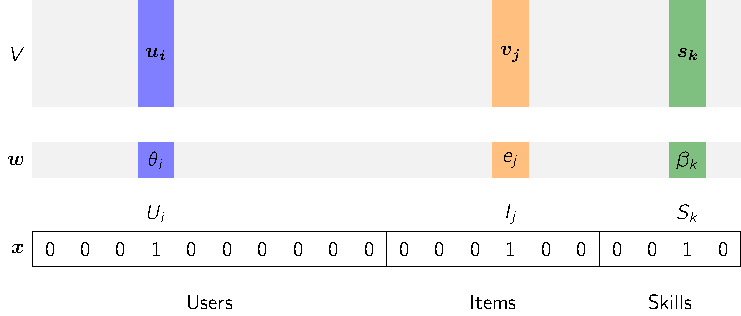
\includegraphics[width=\linewidth]{figures/fm.pdf}
%            If $\psi = \probit$, $w_k, v_{kf} \sim \N(\mu, 1/\lambda)$,\\
  %          $\mu \sim \N(0, 1)$, $\lambda \sim \Gamma(1, 1)$\\
  %          Training using 
        \end{minipage} \hfill %$\rightarrow$ \hfill
        \begin{minipage}{0.49\linewidth}
            \hfill 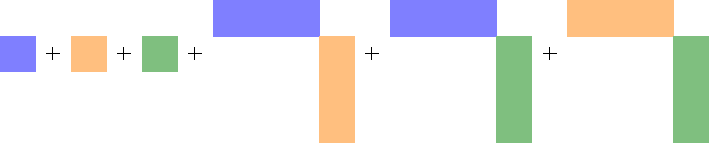
\includegraphics[width=\linewidth]{figures/fm2.pdf}
        \end{minipage}
        \vspace{5mm}

        Existing models are recovered according to the chosen features

        \hspace{5.6cm}\begin{tikzpicture}[xscale=7.8,>=stealth]
        \draw[very thick,<->] (2,0) -- node[above] {IRT} ++(1,0);
        \draw[very thick,<->] (3.05,0) -- node[above] {PFA} ++(1.68,0);
        \end{tikzpicture}
        \begin{center}
        \begin{tabular}{c @{\hspace{1cm}}c cc c ccc c ccc c ccc c ccc c@{\hspace{1cm}} c}
\toprule
\multirow{2}[3]{*}{Triplet} & &  \multicolumn{2}{c}{Users}  & & \multicolumn{3}{c}{Items} & & \multicolumn{3}{c}{Skills}  & & \multicolumn{3}{c}{Wins}  & &  \multicolumn{3}{c}{Fails} & & \multirow{2}[3]{*}{Outcome} \\
\cmidrule{3-4}
\cmidrule{6-8}
\cmidrule{10-12}
\cmidrule{14-16}
\cmidrule{18-20}
&&  1 & 2 & & Q$_1$ & Q$_2$ & Q$_3$ & & S$_1$ & S$_2$ & S$_3$ & & S$_1$ & S$_2$ & S$_3$ & & S$_1$ & S$_2$ & S$_3$ \\
\midrule
$(2, 2, \textnormal{\Uni ✔})$ &&  0 &   1 & &  0 &   1 &   0 &&   1 &   1 &   0 &&   0 &   0 &   0 &&   0 &   0 &   0  && 1 \\
$(2, 2, \textnormal{\Uni ✘})$ &&  0 &   1 & &  0 &   1 &   0 &&   1 &   1 &   0 &&   1 &   1 &   0 &&   0 &   0 &   0  && 0 \\
$(2, 2, \textnormal{\Uni ✔︎})$ &&  0 &   1 & &  0 &   1 &   0 &&   1 &   1 &   0 &&   1 &   1 &   0 &&   1 &   1 &   0  && 1 \\
$(2, 3, \textnormal{\Uni ✘})$ &&  0 &   1 & &  0 &   0 &   1 &&   0 &   1 &   1 &&   0 &   2 &   0 &&   0 &   1 &   0  && 0 \\
$(2, 3, \textnormal{\Uni ✔︎})$ &&  0 &   1 & &  0 &   0 &   1 &&   0 &   1 &   1 &&   0 &   2 &   0 &&   0 &   2 &   1  && 1 \\
$(1, 2, \textnormal{\Uni ✔︎})$ &&  1 &   0 & &  0 &   1 &   0 &&   1 &   1 &   0 &&   0 &   0 &   0 &&   0 &   0 &   0  && 1 \\
$(1, 1, \textnormal{\Uni ✘})$ &&  1 &   0 & &  1 &   0 &   0 &&   0 &   0 &   0 &&   0 &   0 &   0 &&   0 &   0 &   0  && 0 \\
\bottomrule
\end{tabular}

        \end{center}
    }

\end{columns}
\begin{columns}
\column{.61}
\block{Various, large-scale educational datasets}{

    \begin{tabular}{lrrrrrrr}
\toprule
        Name &  Users &  Items &  Skills &  Skills per item &  Entries &  Sparsity &  Attempts per user \\
\midrule
    fraction &    536 &     20 &       8 &            2.800 &    10720 &                  0.000 &              1.000 \\
   timss &    757 &     23 &      13 &            1.652 &    17411 &                  0.000 &              1.000 \\
        ecpe &   2922 &     28 &       3 &            1.321 &    81816 &                  0.000 &              1.000 \\
 assistments &   4217 &  26688 &     123 &            0.796 &   346860 &                  0.997 &              1.014 \\
    berkeley &   1730 &    234 &      29 &            1.000 &   562201 &                  0.269 &              1.901 \\
    castor &  58939 &     17 &       2 &            1.471 &  1001963 &                  0.000 &              1.000 \\
\bottomrule
\end{tabular}
\vspace{1cm}\\
    \begin{minipage}{0.4\linewidth}
    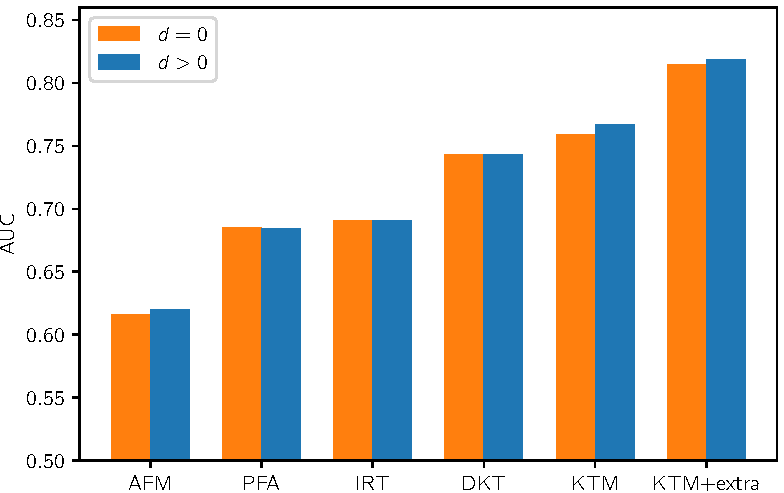
\includegraphics[width=\linewidth]{figures/barchart.pdf}
    \end{minipage}
    \begin{minipage}{0.6\linewidth}
    \begin{tabular}{ccccc}
\toprule
                      model &  dim &             AUC & improvement\\
\midrule
 KTM: items, skills, wins, fails, extra &  5 &  0.819 & \\
 KTM: items, skills, wins, fails, extra &  0 &  0.815 & +0.05 \\
 KTM: items, skills, wins, fails &  10 &  0.767 & \\
 KTM: items, skills, wins, fails &  0 &  0.759 & +0.02 \\
 \emph{DKT} (Wilson et al., 2016) &  100 & 0.743 & +0.05 \\
 IRT: users, items &  0 &  0.691 & \\
 PFA: skills, wins, fails &  0 &  0.685 & +0.07 \\
 AFM: skills, attempts &  0 &  0.616 &\\ \bottomrule
\end{tabular}

    \end{minipage}
    \vspace{1cm}\\
    \begin{tabular}{lllllllll}
\toprule
{} &     AFM &     PFA &              IRT &          MIRTb10 &          MIRTb20 & KTM(iswf0) &      KTM(iswf20) & KTM(iswfe5) \\
\midrule
assistments         &  0.6163 &  0.6849 &           0.6908 &           0.6874 &           0.6907 &     0.7589 &           0.7502 &          \textbf{0.8186} \\
berkeley            &   0.675 &  0.6839 &           0.7532 &           0.7521 &           0.7519 &     0.7753 &  \textbf{0.7780} &          -- \\
ecpe                &      -- &      -- &  \textbf{0.6811} &           0.6807 &  \textbf{0.6810} &         -- &               -- &          -- \\
fraction            &      -- &      -- &           0.6662 &           0.6653 &  \textbf{0.6672} &         -- &               -- &          -- \\
timss           &      -- &      -- &  \textbf{0.6946} &           0.6939 &           0.6932 &         -- &               -- &          -- \\
castor            &      -- &      -- &  \textbf{0.7603} &  \textbf{0.7602} &           0.7599 &         -- &               -- &          -- \\
\bottomrule
\end{tabular}

}


\column{.39}
\block{Findings}{
    \begin{itemize}
    \item It is better to learn a item bias
    \item Side information helps more than latent dimension
    \item We can handle multiple skills per item
    \item We can visualize learning:
    \end{itemize}
    \centering
    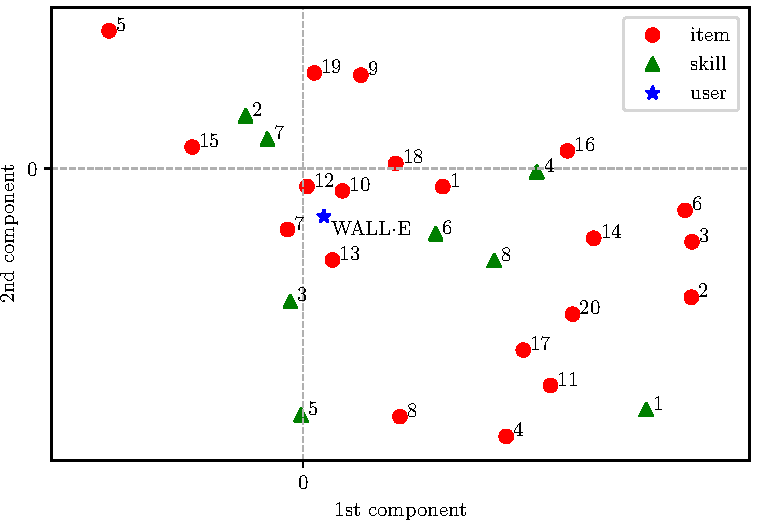
\includegraphics[width=\linewidth]{figures/viz.pdf}
    \vspace{-3cm}
}
\block{References}{
    \printbibliography[heading=none]
}
\end{columns}

\end{document}

\endinput
